%%%%%%%%%%%%%%%%%%%%%%%%%%%%%%%%%%%%%%%%%
% baposter Landscape Poster
% LaTeX Template
% Version 1.0 (11/06/13)
%
% baposter Class Created by:
% Brian Amberg (baposter@brian-amberg.de)
%
% This template has been downloaded from:
% http://www.LaTeXTemplates.com
%
% License:
% CC BY-NC-SA 3.0 (http://creativecommons.org/licenses/by-nc-sa/3.0/)
%
%%%%%%%%%%%%%%%%%%%%%%%%%%%%%%%%%%%%%%%%%

%----------------------------------------------------------------------------------------
%	PACKAGES AND OTHER DOCUMENT CONFIGURATIONS
%----------------------------------------------------------------------------------------

\documentclass[landscape,a1paper,fontscale=0.5]{baposter} % Adjust the font scale/size here

\usepackage[utf8]{inputenc}
\usepackage{graphicx} % Required for including images
\graphicspath{{figures/}} % Directory in which figures are stored

\usepackage{amsmath} % For typesetting math
\usepackage{amssymb} % Adds new symbols to be used in math mode
\usepackage{relsize}
\usepackage{booktabs} % Top and bottom rules for tables
\usepackage{enumitem} % Used to reduce itemize/enumerate spacing
\usepackage{palatino} % Use the Palatino font
\usepackage[font=small,labelfont=bf]{caption} % Required for specifying captions to tables and figures
\usepackage{natbib}

\usepackage{multicol} % Required for multiple columns
\setlength{\columnsep}{1.5em} % Slightly increase the space between columns
\setlength{\columnseprule}{0mm} % No horizontal rule between columns

\usepackage{tikz} % Required for flow chart
\usetikzlibrary{shapes,arrows} % Tikz libraries required for the flow chart in the template

\newcommand{\compresslist}{ % Define a command to reduce spacing within itemize/enumerate environments, this is used right after \begin{itemize} or \begin{enumerate}
\setlength{\itemsep}{1pt}
\setlength{\parskip}{0pt}
\setlength{\parsep}{0pt}
}

\definecolor{lightblue}{rgb}{0.145,0.6666,1} % Defines the color used for content box headers

\begin{document}

\begin{poster}
{
headerborder=closed, % Adds a border around the header of content boxes
colspacing=1em, % Column spacing
bgColorOne=white, % Background color for the gradient on the left side of the poster
bgColorTwo=white, % Background color for the gradient on the right side of the poster
borderColor=lightblue, % Border color
headerColorOne=black, % Background color for the header in the content boxes (left side)
headerColorTwo=lightblue, % Background color for the header in the content boxes (right side)
headerFontColor=white, % Text color for the header text in the content boxes
boxColorOne=white, % Background color of the content boxes
textborder=roundedleft, % Format of the border around content boxes, can be: none, bars, coils, triangles, rectangle, rounded, roundedsmall, roundedright or faded
eyecatcher=true, % Set to false for ignoring the left logo in the title and move the title left
headerheight=0.1\textheight, % Height of the header
headershape=roundedright, % Specify the rounded corner in the content box headers, can be: rectangle, small-rounded, roundedright, roundedleft or rounded
headerfont=\Large\bf\textsc, % Large, bold and sans serif font in the headers of content boxes
%textfont={\setlength{\parindent}{1.5em}}, % Uncomment for paragraph indentation
linewidth=2pt % Width of the border lines around content boxes
}
%----------------------------------------------------------------------------------------
%	TITLE SECTION 
%----------------------------------------------------------------------------------------
%
{\includegraphics[height=4em]{logo.png}} % First university/lab logo on the left
{\bf\textsc{Restricted Boltzmann Machine}\vspace{0.5em}} % Poster title
{\textsc{\{ Chaïmaa Kadaoui, Othman Sbai and Xi Shen \} \hspace{12pt} MVA - ENS Paris Saclay}} % Author names and institution
{\includegraphics[height=4em]{logo.png}} % Second logo on the right - Ecole des Ponts

%----------------------------------------------------------------------------------------
%	DEFINITION
%----------------------------------------------------------------------------------------

\headerbox{Definition}{name=definition,column=0,row=0}{

A Restricted Boltzman Machine is an undirected graph which can be decomposed in two layers.
\begin{center}

\includegraphics[width=0.75\linewidth]{rbm}
\end{center}
It is \emph{restricted} because no connection between nodes of the same layer is supposed. The matrix $W$ characterizes the connections between the two layers. For simplification, we suppose that the variables $ \mathbf{x} $ and $ \mathbf{h} $ are binary. This model is called Bernoulli RBM.

The hidden variables can be seen as features and the goal of the RMB is to represent meaningful features.

%\vspace{0.3em} % When there are two boxes, some whitespace may need to be added if the one on the right has more content
}

%----------------------------------------------------------------------------------------
%	ENERGY AND PROBABILITY
%----------------------------------------------------------------------------------------

\headerbox{Energy and Probability}{name=energy,column=1,row=0,bottomaligned=definition}{

We introduce the two bias vectors $c$ and $b$ to define the energy of this graph:

\[ E(x,h) = -h^\top W x - c^\top x - b^\top h \]

We can write the joint probability of $ \mathbf{x} $ and $ \mathbf{h} $ as: 

\[ p(x,h) = \exp(-E(x,h)) / Z \]

$Z$ is the partition parameter which can be computed by calculating all the possibles values of $ \mathbf{x} $  and $ \mathbf{h} $ . In practice, this parameter is intractable. 

\textbf{Inference} We can prove that given $\mathbf{x}$, $h_j$ follows a Bernoulli: $$p(h_j=1|x) = sigm(b_j + W_{j.}x)$$
$ W_{j.}$ is the j-th row of $W$ and $sigm$ defines the sigmoid function.
}


%----------------------------------------------------------------------------------------
%	CONTRASTIVE DIVERGENCE
%----------------------------------------------------------------------------------------

\headerbox{Contrastive Divergence}{name=CD,column=0,span=2,row=0,below=definition}{


To train the RBM with our data $\mathbf{x}^{(t)}$, we would like to minimize the average loss:
$ \frac{1}{T} \sum_t l(f(\mathbf{x}^{(t)})) =  \frac{1}{T} \sum_t - \log p(\mathbf{x}^{(t)}) $

We will apply a stochastic gradient descent. We derive each term of the sum with respect to our model parameter $\theta$ as follow (where $\mathbb{E}_h$ and $\mathbb{E}_{x,h}$ are expectations of $h$ and $(x,h)$ respectively):

\[ \frac{\partial - \log p(\mathbf{x}^{(t)})}{\partial \theta} = \mathbb{E}_h \left[ \frac{\partial E(\mathbf{x}^{(t)} ,h)}{\partial \theta} | \mathbf{x}^{(t)} \right] - \mathbb{E}_{x,h} \left[ \frac{\partial E(\mathbf{x} ,h)}{\partial \theta} \right] \]

The first term is called the \emph{positive phase} and the second term the \emph{negative phase}. Because of the difficulty to compute the second term, we will use an algorithm called \emph{Contrastive Divergence}. The key points of the algorithm are:

\begin{itemize}
	\itemsep=-0.02em
	\item We estimate the expectation $\mathbb{E}_{x,h}$ by sampling a single point $\mathbf{\tilde x}$.
	\item To do so, we use Gibbs sampling in chain (we apply it $k$ times).
	\item We initialize our Gibbs sampling with $\mathbf{x^{(t)}}$.
	\item Update parameters W, b, c; with $h(x) = p(h|x) = sigm(b + Wx)$ and $\alpha$ the learning rate.
	    \begin{itemize}\compresslist
		\item $ W = W + \alpha \left( h(\mathbf{x^{(t)}})\mathbf{x^{(t)}}^\top - h(\mathbf{\tilde x})\mathbf{\tilde x}^\top \right) $
		\item $ b = b + \alpha \left(h(\mathbf{x^{(t)}}) - h(\mathbf{\tilde x}) \right) $
		\item $ c = c + \alpha \left(\mathbf{x^{(t)}} - \mathbf{\tilde x} \right) $
		\end{itemize}
\end{itemize}
}


%----------------------------------------------------------------------------------------
%	RESULTS on MNIST
%----------------------------------------------------------------------------------------

\headerbox{Results On MNIST data}{name=resultsMNIST,column=2,span=2}{ % This block's bottom aligns with the bottom of the conclusion block
We implemented the RBM training algorithm both using numpy and using tensorflow, we applied it to the MNIST dataset (images of handwritten digits). In the case of image data, each pixel is considered as a node; the intensity $p \in [0,1]$ of a pixel is considered as a probability. \\

The left figure is the evolution of the average stochastic reconstruction $\lVert \mathbf{x^{(t)}} - \mathbf{\tilde{x}} \rVert^2$ for both the training and the test dataset at each iteration. The right figure is the visualization of the connections between one hidden unit and each element of the input vector.

\begin{center}
\begin{minipage}{7.5in}
	\centering
	\raisebox{-0.5\height}{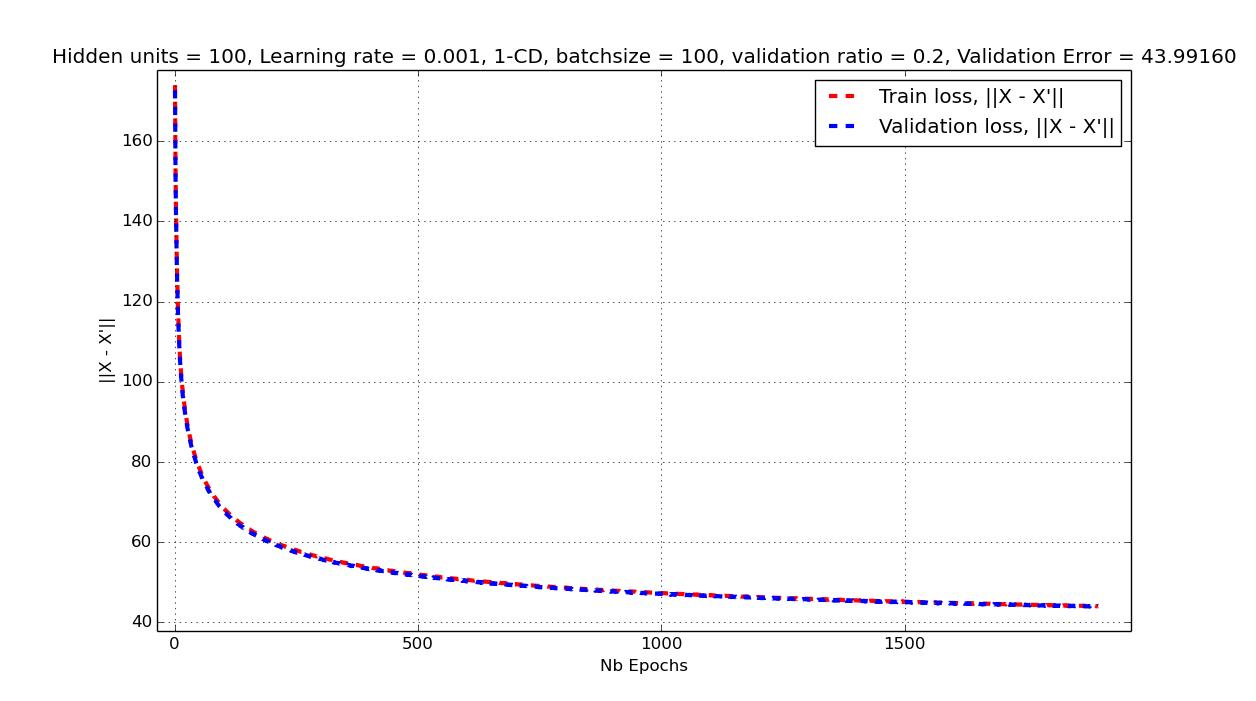
\includegraphics[width=0.47\linewidth]{TrainCurve}}
	\hspace*{.2in}
	\raisebox{-0.5\height}{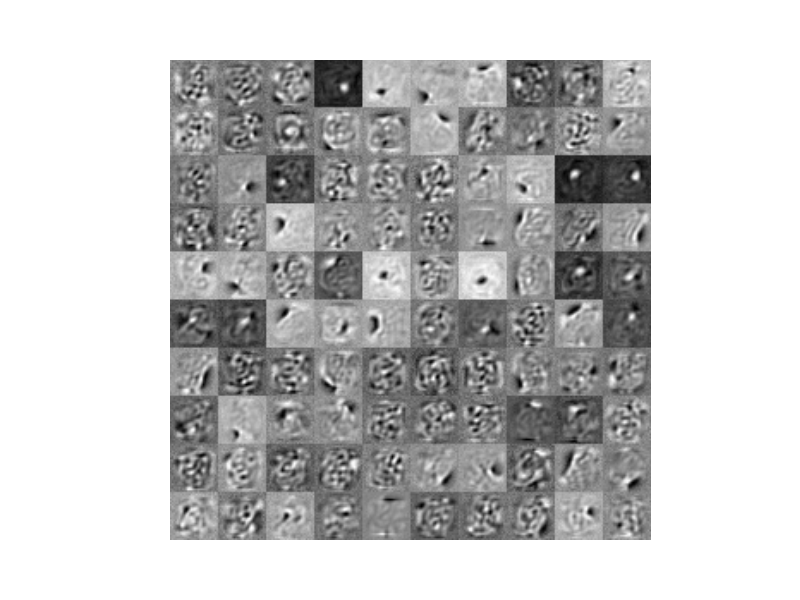
\includegraphics[width=0.47\linewidth]{MNIST_Filter_20Epochs}}
\end{minipage}
\end{center}


%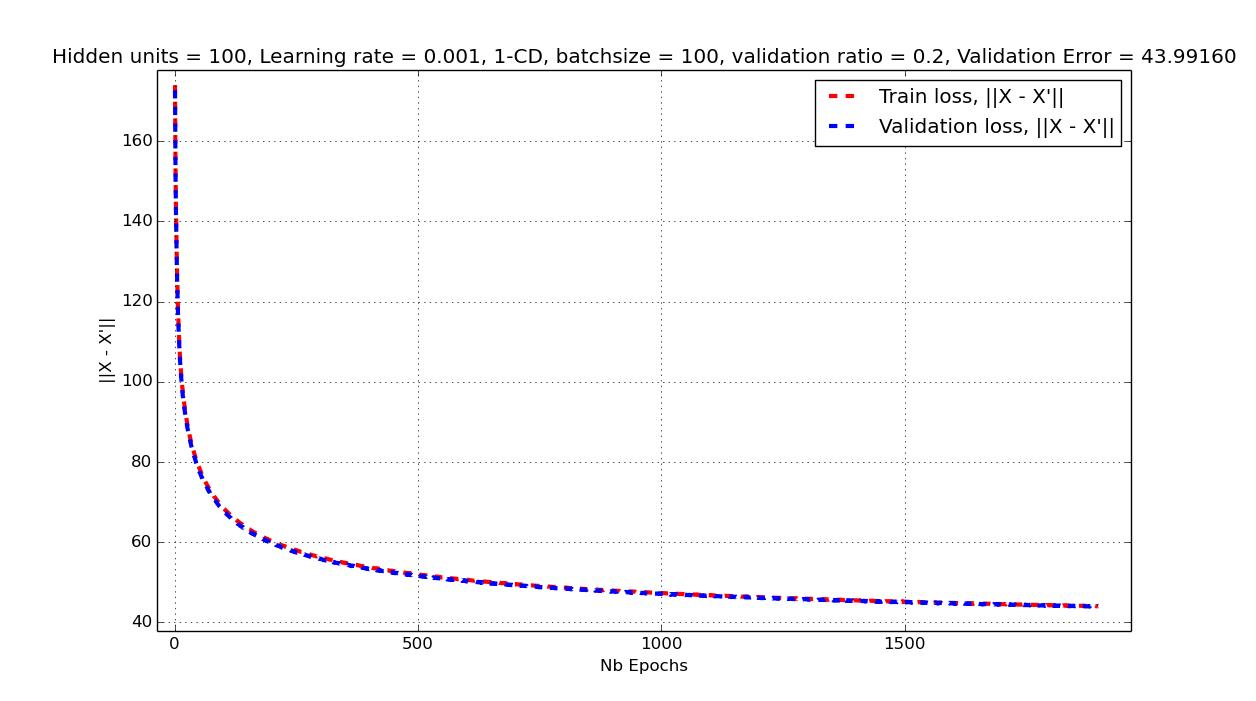
\includegraphics[width=0.5\linewidth]{TrainCurve}
%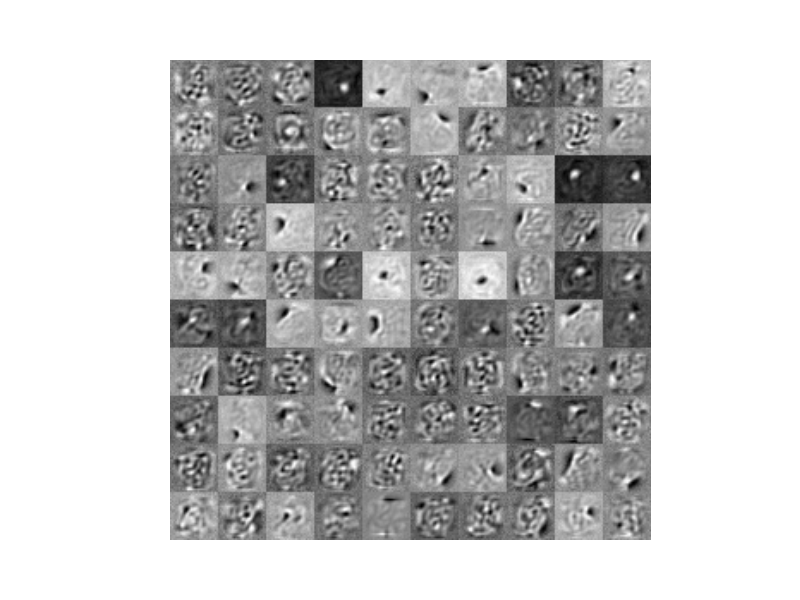
\includegraphics[width=0.5\linewidth]{MNIST_Filter_20Epochs}
%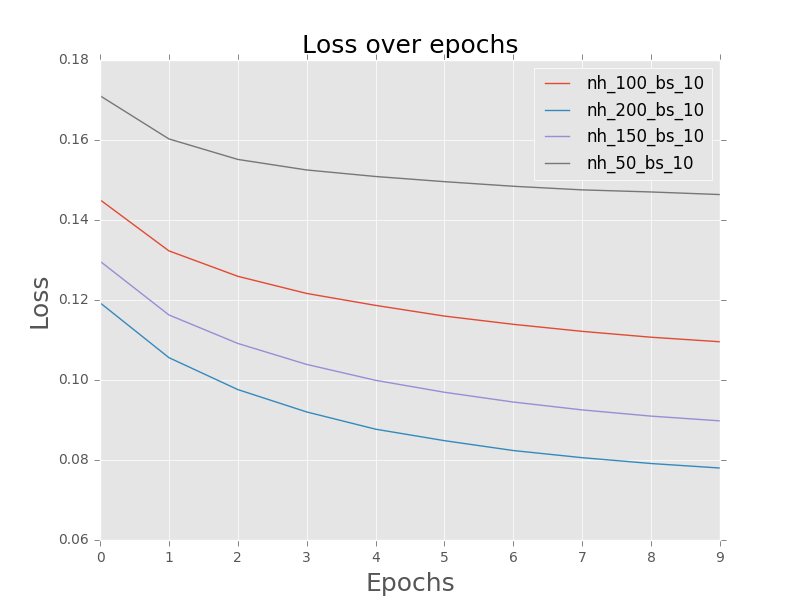
\includegraphics[width=0.5\linewidth]{MNIST_LossOverEpochs_NHidden}
%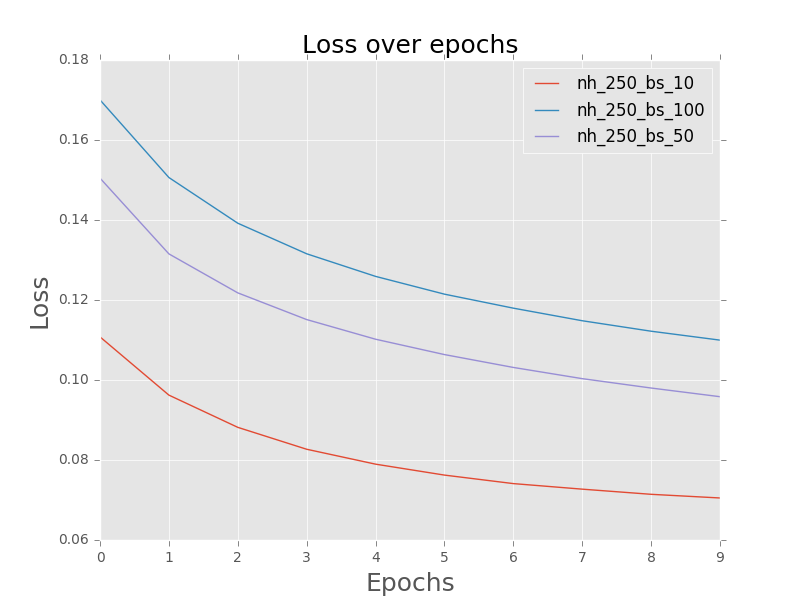
\includegraphics[width=0.5\linewidth]{MNIST_LossOverEpochs_BatchSize}
%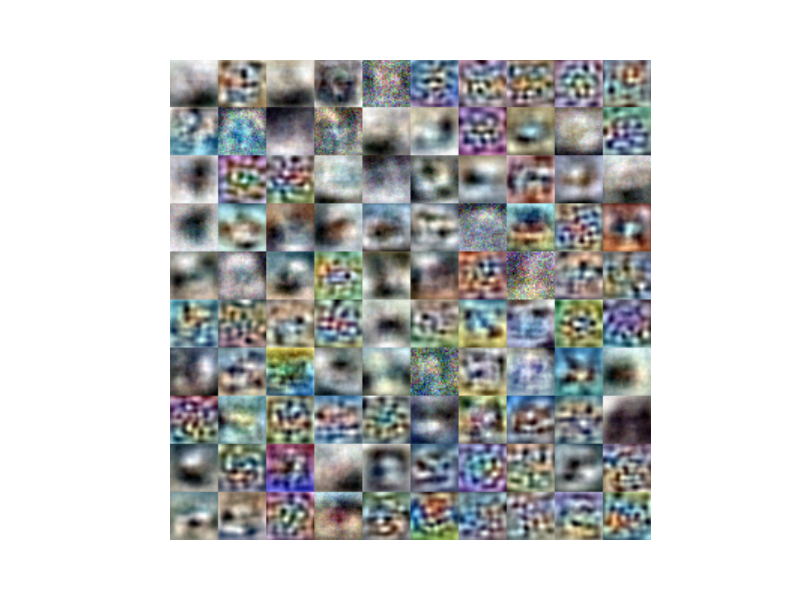
\includegraphics[width=0.5\linewidth]{CIFAR_LearnedWeights}
}

%----------------------------------------------------------------------------------------
%	RESULTS on CIFAR
%----------------------------------------------------------------------------------------

\headerbox{Results On CIFAR data}{name=resultsCIFAR,column=2,span=2,below=resultsMNIST}{ % This block's bottom aligns with the bottom of the conclusion block

Using tensorflow, we applied the algorithm to the CIFAR dataset (a dataset of colour images in different classes).\\

The left figure is the evolution of the average stochastic reconstruction at each iteration for different settings of the algorithm. The right figure is the visualization of the connections between one hidden unit and each element of the input vector.

\begin{center}
	\begin{minipage}{7.5in}
		\centering
		\raisebox{-0.5\height}{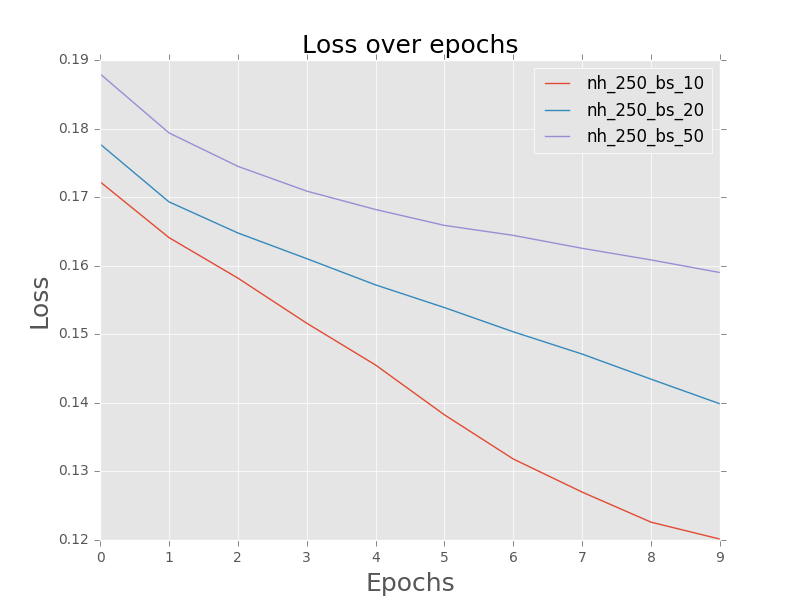
\includegraphics[width=0.47\linewidth]{CIFAR_LossOverEpochs_BatchSize}}
		\hspace*{.2in}
		\raisebox{-0.5\height}{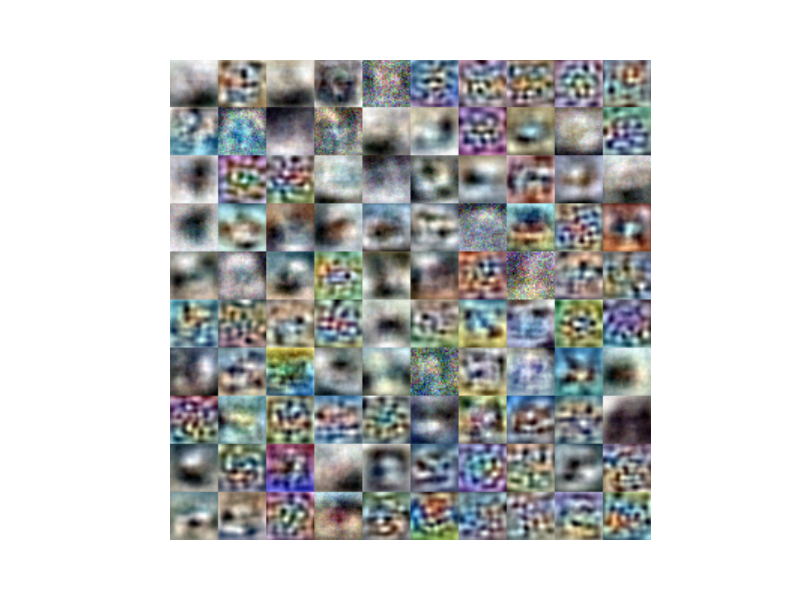
\includegraphics[width=0.47\linewidth]{CIFAR_LearnedWeights}}
	\end{minipage}
\end{center}

%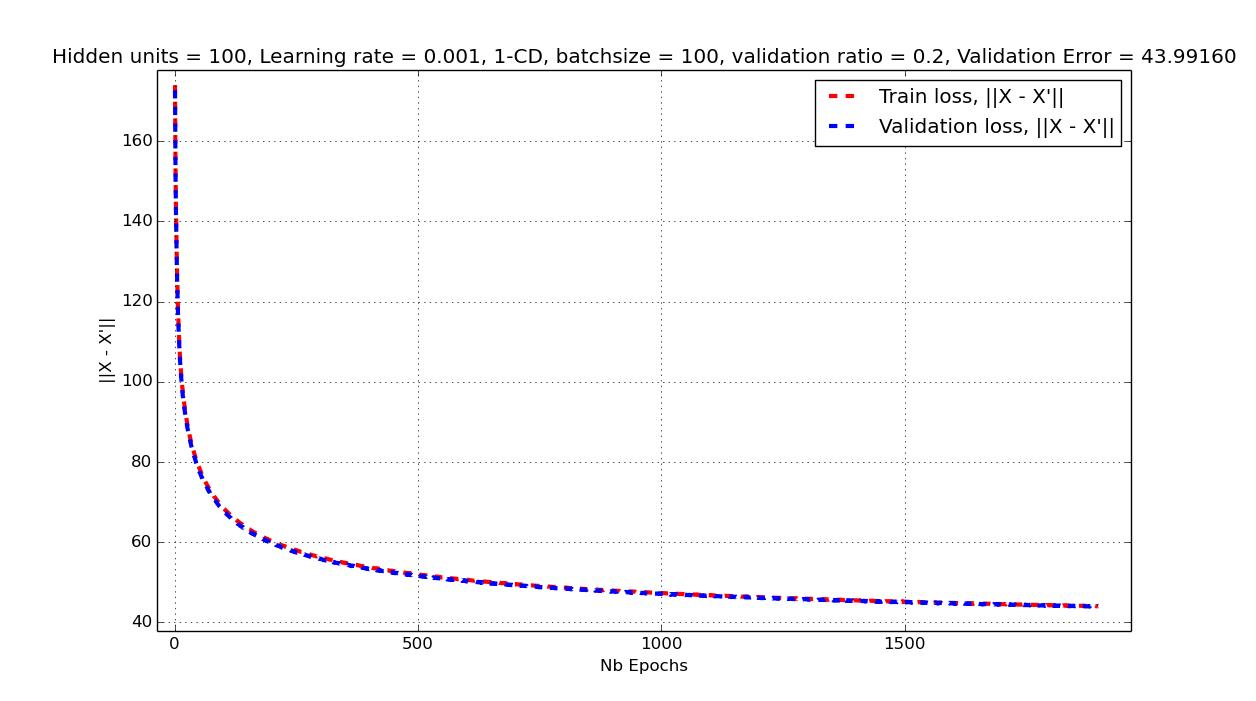
\includegraphics[width=0.5\linewidth]{TrainCurve}
%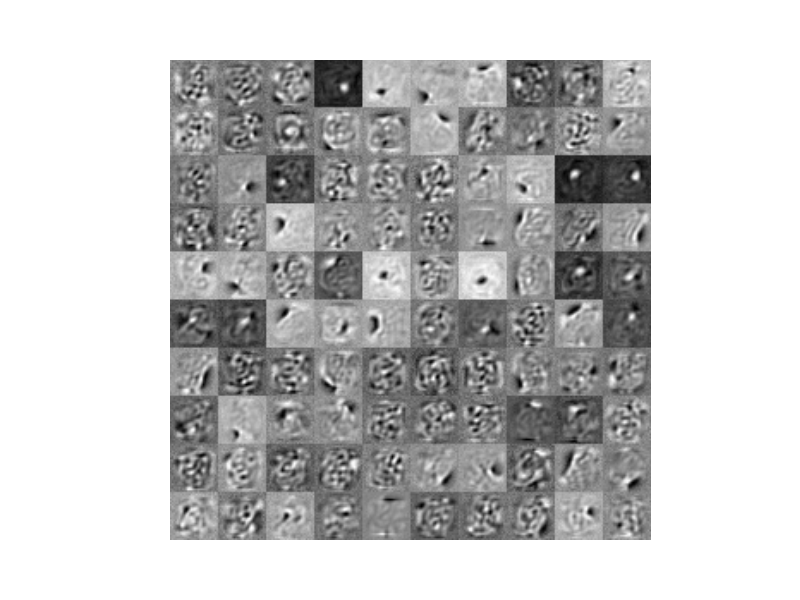
\includegraphics[width=0.5\linewidth]{MNIST_Filter_20Epochs}
%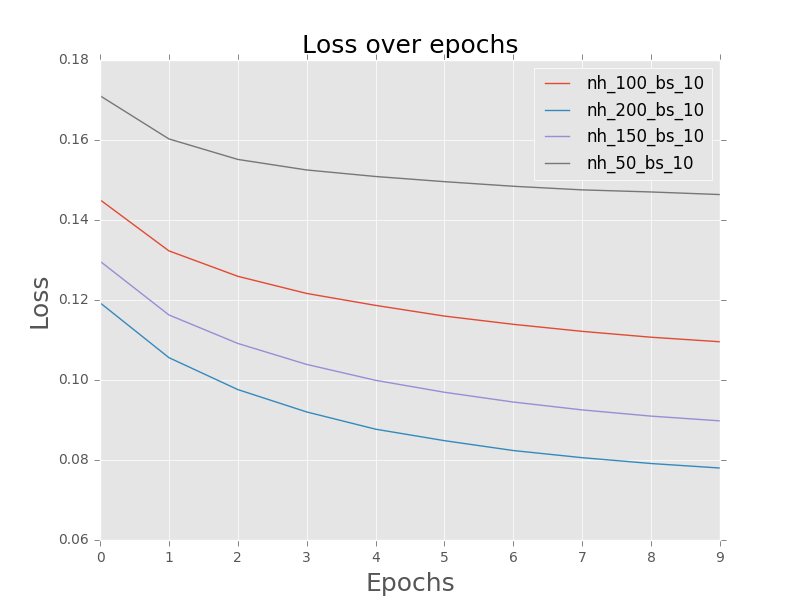
\includegraphics[width=0.5\linewidth]{MNIST_LossOverEpochs_NHidden}
%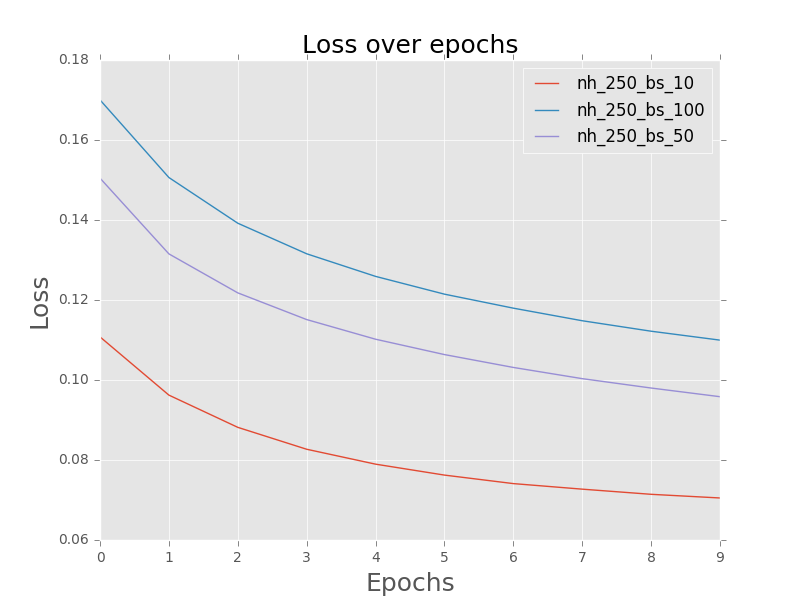
\includegraphics[width=0.5\linewidth]{MNIST_LossOverEpochs_BatchSize}
%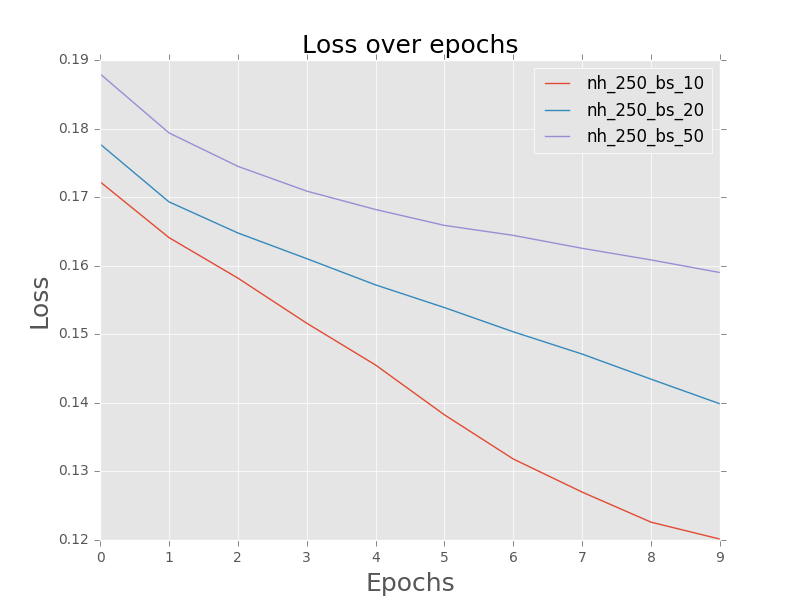
\includegraphics[width=0.5\linewidth]{CIFAR_LossOverEpochs_BatchSize}
%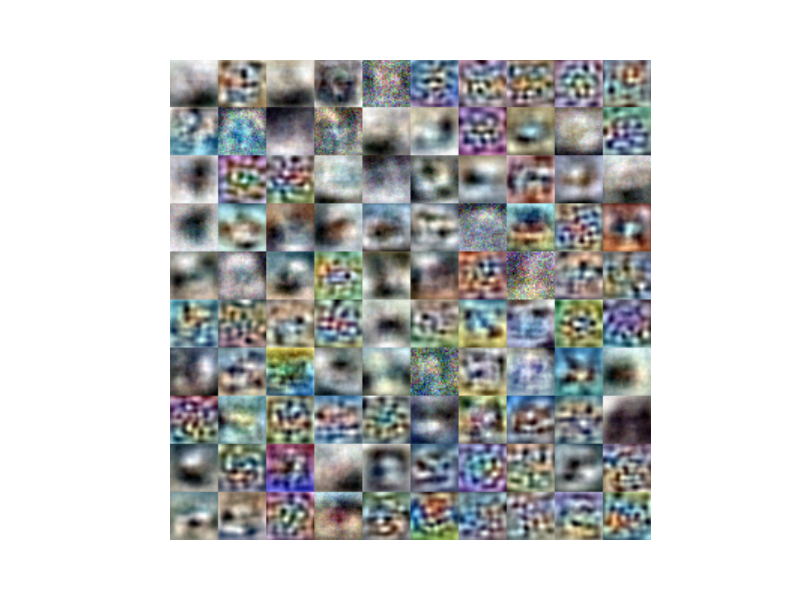
\includegraphics[width=0.5\linewidth]{CIFAR_LearnedWeights}


}


%----------------------------------------------------------------------------------------
%	REFERENCES
%----------------------------------------------------------------------------------------

\headerbox{References}{name=references,column=0,span=2,above=bottom}{

\renewcommand{\section}[2]{\vskip 0.05em} % Get rid of the default "References" section title
\nocite{*} % Insert publications even if they are not cited in the poster
\small{ % Reduce the font size in this block
\bibliographystyle{plain}
\bibliography{biblio} % Use biblio.bib as the bibliography file
}}



%----------------------------------------------------------------------------------------
%	APPLICATIONS
%----------------------------------------------------------------------------------------

\headerbox{Applications of RBM}{name=applications,column=0,span=2,below=CD, above=references}{ % This block is as tall as the references block

\begin{multicols}{2}
	\begin{itemize}\compresslist
		\item RBM is a generative model, but it can be used to improve classification tasks: instead of training on the raw data $\mathbf{x}$, we can use the learnt matrix of connections $W$.
		\item RBM are also used for collaborative filtering: given a set of N users and M movies, we would like to recommend movies to the users.
		\item RBM are helpful for computer vision tasks such as object recognition, image denoising and inpainting.
	\end{itemize}
\end{multicols}

}

%----------------------------------------------------------------------------------------
%	CONCLUSION
%----------------------------------------------------------------------------------------

\headerbox{Conclusion}{name=conclusion,column=2,span=2,above=bottom}{

\begin{multicols}{2}
\begin{itemize}\compresslist
%\item As for other deep learning techniques, RBM implementations are costly. The use of GPU achitectures is necessary.
\item Increasing the number of hidden layers improves the performances but rises the time complexity. We found that about 250 hidden layers is a good trade-off for the MNIST and CIFAR datasets.
\item The more steps we use for Gibbs sampling, the lower is the bias of our estimate. However it takes more time to compute. An alternative of the Contrastive Divergence algorithm is called Persistent Contrastive Divergence: at each iteration of the algorithm, we initialize the Gibbs sampling with the sample from the previous iteration.
\item It is possible to adapt the RBM model for unbounded reals by adding a quadratic term ($\frac{1}{2}\mathbf{x}^\top \mathbf{x}$) to the energy. Then, $p(\mathbf{x}|h)$ becomes a Gaussian distribution. This is called Gaussian-Bernoulli RBM.
\end{itemize}
\end{multicols}


}


%----------------------------------------------------------------------------------------

\end{poster}

\end{document}